\documentclass[fleqn]{article}
\usepackage[left=2cm,top=2cm,right=2cm,bottom=2cm]{geometry}
\usepackage{graphicx}
\usepackage{amsmath}
\usepackage{amssymb}
\usepackage{tikz}
\usepackage{subcaption}
\usetikzlibrary{}

\newcommand{\bigCI}{\mathrel{\text{\scalebox{1.07}{$\perp\mkern-10mu\perp$}}}}

\title{CS6790: Geometry \& Photometry-based Computer Vision \\ Assignment-2 (Finding Intrinsic parameters)}
\author{Arulkumar S (CS15D202)}
\date{}

\begin{document} 
\maketitle
\section{Finding intrinsic parameters (Assuming full K matrix)}
\subsection{by using 5 perpendicularity relations between vanishing points}
\subsubsection{Procedure}
 
\begin{enumerate} 
  \item The intrinsic parameters shall be determined using 5 sets of perpendicular vanishing points.
  \item To get 5 sets of vanishing points, the given chess board images (5) are used. To get the vanishing vanishing point, the perpendicular
  pair of parallel lines in the chess board are used. refer to the Figure \ref{chessboard_perpendicular}.  Let the set of of points to deniote
  the parallel lines in one direction be $P_{l_1}, P_{l_2}, P_{l_3}, P_{l_4}$. Let the other set of points selected to denote the parallel lines in
  perpendicular direction be $P_{m_1}, P_{m_2}, P_{m_3}, P_{m_4}$.
  \item The vanishing point is determined from the set of chosen points as follows:
  \begin{eqnarray*}
  \begin{aligned}
  \text{vanishing point 1,} VP_1 &= (P_{l_1} \times P_{l_2}) \times (P_{l_3} \times P_{l_4})\\
  \text{vanishing point 2,} VP_2 &= (P_{m_1} \times P_{m_2}) \times (P_{m_3} \times P_{m_4})\\
  \end{aligned}
  \end{eqnarray*} 
  
 \item Since the vanishing points $VP_1, VP_2$ are perpendicular, we can form an equation with $\Psi = K^{-T}K^{-1}$, with $K$ being the matrix of
 camera intrinsic parameters as follows:
  \begin{eqnarray*}
  \begin{aligned}
  (VP_1)^T \Psi (VP_2) = 0
  \end{aligned}
  \end{eqnarray*}
  The $K$ matrix has 5 free parameters as follows:
  \[
   \begin{bmatrix}
   		f_x & s & u_x \\
   		0 & f_y & u_y \\
   		0 & 0 & 1
   \end{bmatrix}
  \]
  where  $f_x, f_y $ = focal length in $x, y$ direction respectively, $u_x, u_y$ = camera center, $s$ = skew parameter.
  
  \item With 5 sets of perpendicular vanishing points, we can get 5 such equation as given in step 4 above.
  \begin{eqnarray*}
  \begin{aligned}
  \begin{bmatrix}
  x_{l1}x_{m1} &  (x_{l1}y_{m1} + y_{l1}x_{m1}) & (x_{l1}h_{m1} + h_{l1}x_{m1}) & y_{l1}y_{m1} & (y_{l1}h_{m1} + h_{l1}y_{m1}) & h_{l1}h_{m1}\\
  x_{l2}x_{m2} &  (x_{l2}y_{m2} + y_{l2}x_{m2}) & (x_{l2}h_{m2} + h_{l2}x_{m2}) & y_{l2}y_{m2} & (y_{l2}h_{m2} + h_{l2}y_{m2}) & h_{l2}h_{m2}\\
  \vdots
  \end{bmatrix}
  \begin{bmatrix}
  a \\ b \\ c\\ d\\ e\\ f
  \end{bmatrix} = 0
  \end{aligned}
  \end{eqnarray*}
 
  here, 
  \begin{eqnarray*}
  \begin{aligned}
  \Psi = \begin{bmatrix}
   		a & b & c \\
   		b & d & e \\
   		c & e & f
   \end{bmatrix}
  \end{aligned}
  \end{eqnarray*}
  \item The parameters shall be determined using the Singular value decomposition (SVD). i.e., the singular vector corresponding to the least singular
  value is the solution for $\Psi$.
  \item Once $\Psi$ is determined, we can use Cholesky decomposition to get the intrinsic camera paramerters $K$. 
  The $K$ matrix has 5 free parameters as follows:
  \[
   \begin{bmatrix}
   		f_x & s & u_x \\
   		0 & f_y & u_y \\
   		0 & 0 & 1
   \end{bmatrix}
  \]
  where  $f_x, f_y $ = focal length in $x, y$ direction respectively, $u_x, u_y$ = camera center, $s$ = skew parameter.

\item \textbf{Result (chess board images of size $600 \times 400 \text{ pixels}$)}:

\[
 K = \begin{bmatrix}
   		f_x & s & u_x \\
   		0 & f_y & u_y \\
   		0 & 0 & 1
   \end{bmatrix}
=    \begin{bmatrix}
   		1191.2 & 8.2 & 326.2 \\
   		0 & 811.3 & 153.6 \\
   		0 & 0 & 1
   \end{bmatrix}
\]

\end{enumerate}

\begin{figure}[!ht]
\centering
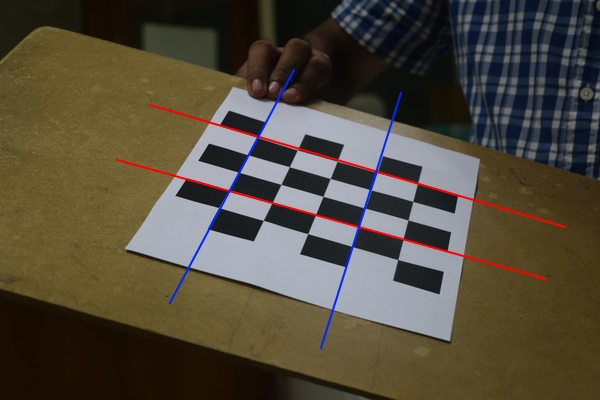
\includegraphics[scale=0.4]{./pics/cb1_perp}
\caption{The perpendicular pair of parallel lines chosen to get the perpendicular rays from 2 vanishing points \label{chessboard_perpendicular}}
\end{figure}

\subsection{by computing the homography relation between metric co-ordinate system fixed to scene plane \& image}
\subsubsection{Procedure}
\begin{itemize}
\item The chess board images are used to find the homography between scene coordinates and the image coordinates.
\item consider $H$ as the homography matrix that transforms the scene coordinates to image coordinates. 
\item Consider transforming the circular points $I(1, +i, 0)$, $J(1, -i, 0)$ to the image co-ordinates. Since the points $I, J$
which are lying in Absolute Conic of 3D space are transformed to the points on the Image of Absolute Conic (IAC) in the 2D image plane (
($\Psi$), each homography gives two contraints. ($h_1 \Psi h_1 = h_2 \Psi h_2$, $h_1^T \Psi h_2 = 0$).
\item Hence, 3 such homographies give 6 constraint equations which are used to solve for the parameters of $\Psi = K^{-T}K^{-1}$.
  here, 
  \begin{eqnarray*}
  \begin{aligned}
  \Psi = \begin{bmatrix}
   		a & b & c \\
   		b & d & e \\
   		c & e & f
   \end{bmatrix}
  \end{aligned}
  \end{eqnarray*}
  \item To find 3 homographies, the chess board images are considered such that the scene points $(0, 0, 1),(0, 1, 1),(1, 1, 1),(1, 0, 1)$ are
  transformed to image co-ordinates which are selected appropriately.
  \item The parameters shall be determined using the Singular value decomposition (SVD). i.e., the singular vector corresponding to the least singular
  value is the solution for $\Psi$.
  \item Once $\Psi$ is determined, we can use Cholesky decomposition to get the intrinsic camera paramerters $K$. 
  The $K$ matrix has 5 free parameters as follows:
  \[
   \begin{bmatrix}
   		f_x & s & u_x \\
   		0 & f_y & u_y \\
   		0 & 0 & 1
   \end{bmatrix}
  \]
  where  $f_x, f_y $ = focal length in $x, y$ direction respectively, $u_x, u_y$ = camera center, $s$ = skew parameter.


\item \textbf{Result (chess board images of size $600 \times 400 \text{ pixels}$)}:

\[
 K = \begin{bmatrix}
   		f_x & s & u_x \\
   		0 & f_y & u_y \\
   		0 & 0 & 1
   \end{bmatrix}
=    \begin{bmatrix}
   		1459.45 & 4.2 & 458.2 \\
   		0 & 834.35 & 220.5 \\
   		0 & 0 & 1
   \end{bmatrix}
\]

The calculation was very sensitive to the selection of points. i.e., most of the times, it gives ``matrix not positive definite'' error during Cholesky
factorization.

\item \textbf{Result (triple box image of size $890 \times 738 \text{ pixels}$)}:

\[
 K = \begin{bmatrix}
   		f_x & s & u_x \\
   		0 & f_y & u_y \\
   		0 & 0 & 1
   \end{bmatrix}
=    \begin{bmatrix}
   		1738.5 & 4.6 & 562.2 \\
   		0 & 1310.5 & 468.6 \\
   		0 & 0 & 1
   \end{bmatrix}
\]
\end{itemize}

\section{By assuming square pixels (i.e. skew = 0 and $f x = f y$)}

By assuming the skew  = 0 \& $f_x = f_y$, the intrinsic camera parameters are reduced to 3. i.e., the  number of constraint equations are reduced.
The intrinsic camera parameter matrix can be defined as,
\[
   \begin{bmatrix}
   		f & 0 & u_x \\
   		0 & f & u_y \\
   		0 & 0 & 1
   \end{bmatrix}
\]

\subsection{by using 3 perpendicularity relations between vanishing points}
\subsubsection{Procedure}
\begin{itemize}

  \item The intrinsic parameters shall be determined using 3 sets of perpendicular vanishing points, as $f_x = f_y$ and $skew = 0$..
  \item To get 3 sets of vanishing points, the given chess board images (3) are used. To get the vanishing vanishing point, the perpendicular
  pair of parallel lines in the chess board are used. refer to the Figure \ref{chessboard_perpendicular}.  Let the set of of points to deniote
  the parallel lines in one direction be $P_{l_1}, P_{l_2}, P_{l_3}, P_{l_4}$. Let the other set of points selected to denote the parallel lines in
  perpendicular direction be $P_{m_1}, P_{m_2}, P_{m_3}, P_{m_4}$.
  \item The vanishing point is determined from the set of chosen points as follows:
  \begin{eqnarray*}
  \begin{aligned}
  \text{vanishing point 1,} VP_1 &= (P_{l_1} \times P_{l_2}) \times (P_{l_3} \times P_{l_4})\\
  \text{vanishing point 2,} VP_2 &= (P_{m_1} \times P_{m_2}) \times (P_{m_3} \times P_{m_4})\\
  \end{aligned}
  \end{eqnarray*} 
  
 \item Since the vanishing points $VP_1, VP_2$ are perpendicular, we can form an equation with $\Psi = K^{-T}K^{-1}$, with $K$ being the matrix of
 camera intrinsic parameters as follows:
  \begin{eqnarray*}
  \begin{aligned}
  (VP_1)^T \Psi (VP_2) = 0
  \end{aligned}
  \end{eqnarray*}
  The $K$ matrix has 3 free parameters as follows:
  \[
   \begin{bmatrix}
   		f & 0 & u_x \\
   		0 & f & u_y \\
   		0 & 0 & 1
   \end{bmatrix}
  \]
  where  $f$ = focal length, $u_x, u_y$ = camera center.
  
  \item With 3 sets of perpendicular vanishing points, we can get 3 such equation as given in step 4 above.
  \begin{eqnarray*}
  \begin{aligned}
  \begin{bmatrix}
  x_{l1}x_{m1} + y_{l1}y_{m1} & (x_{l1}h_{m1} + h_{l1}x_{m1}) & (y_{l1}h_{m1} + h_{l1}y_{m1}) & h_{l1}h_{m1}\\
  x_{l2}x_{m2} + y_{l2}y_{m2} & (x_{l2}h_{m2} + h_{l2}x_{m2})  & (y_{l2}h_{m2} + h_{l2}y_{m2}) & h_{l2}h_{m2}\\
  \vdots
  \end{bmatrix}
  \begin{bmatrix}
  a \\ c\\ e\\ f
  \end{bmatrix} = 0
  \end{aligned}
  \end{eqnarray*}
 
  here, 
  \begin{eqnarray*}
  \begin{aligned}
  \Psi = \begin{bmatrix}
   		a & 0 & c \\
   		0 & a & e \\
   		c & e & f
   \end{bmatrix}
  \end{aligned}
  \end{eqnarray*}
  \item The parameters shall be determined using the Singular value decomposition (SVD). i.e., the singular vector corresponding to the least singular
  value is the solution for $\Psi$.
  \item Once $\Psi$ is determined, we can use Cholesky decomposition to get the intrinsic camera paramerters $K$. 

\item \textbf{Result}:

\begin{figure}[!ht]
\centering
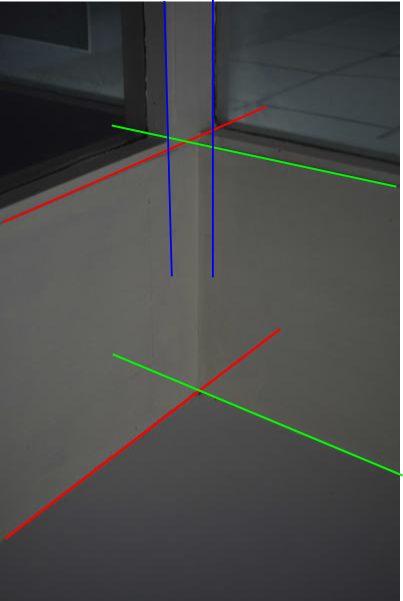
\includegraphics[scale=0.4]{./pics/img1_ink}
\caption{The perpendicular pair of parallel lines chosen to get the perpendicular rays from 3 vanishing points $(400 \times 600 image)$}
\end{figure}
\[
 K = \begin{bmatrix}
   		f & 0 & u_x \\
   		0 & f & u_y \\
   		0 & 0 & 1
   \end{bmatrix}
=    \begin{bmatrix}
   		708.3 & 0 & 188.3 \\
   		0 & 708.3 & 452.2 \\
   		0 & 0 & 1
   \end{bmatrix}
\]

\clearpage
\begin{figure}[!ht]
\centering
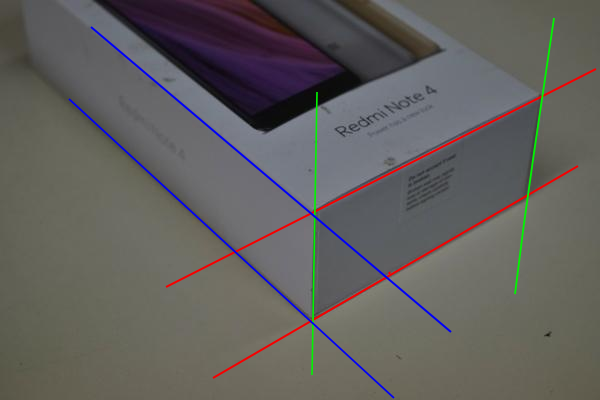
\includegraphics[scale=0.4]{./pics/img2_ink}
\caption{The perpendicular pair of parallel lines chosen to get the perpendicular rays from 3 vanishing points $(600 \times 400 image)$}
\end{figure}
\[
 K = \begin{bmatrix}
   		f & 0 & u_x \\
   		0 & f & u_y \\
   		0 & 0 & 1
   \end{bmatrix}
=    \begin{bmatrix}
   		1333.36 & 0 & 137.8 \\
   		0 & 1333.36 & 389.2 \\
   		0 & 0 & 1
   \end{bmatrix}
\]
\end{itemize}

\subsection{by computing the homography relation between metric co-ordinate system fixed to scene plane \& image}
\subsubsection{Procedure}
\begin{itemize}
\item As we have seen in the question 1, one homography calculation gives us 2 constraints. Hence, 2 such homographies give 
4 constraint equations which are used to solve for the parameters of $\Psi = K^{-T}K^{-1}$.
  here, 
  \begin{eqnarray*}
  \begin{aligned}
  \Psi = \begin{bmatrix}
   		a & 0 & c \\
   		0 & a & e \\
   		c & e & f
   \end{bmatrix}
  \end{aligned}
  \end{eqnarray*}
  \item The parameters shall be determined using the Singular value decomposition (SVD). i.e., the singular vector corresponding to the least singular
  value is the solution for $\Psi$.
  \item Once $\Psi$ is determined, we can use Cholesky decomposition to get the intrinsic camera paramerters $K$. 
  The $K$ matrix has 3 free parameters as follows:
  \[
   \begin{bmatrix}
   		f & 0 & u_x \\
   		0 & f & u_y \\
   		0 & 0 & 1
   \end{bmatrix}
  \]
  where  $f$ = focal length, $u_x, u_y$ = camera center.

\item \textbf{Result (chess board images of size $600 \times 400 \text{ pixels}$)}:

\[
 K = \begin{bmatrix}
   		f & 0 & u_x \\
   		0 & f & u_y \\
   		0 & 0 & 1
   \end{bmatrix}
=    \begin{bmatrix}
   		1382.8 & 0 & 358.2 \\
   		0 & 1382.8 & 160.5 \\
   		0 & 0 & 1
   \end{bmatrix}
\]

\item \textbf{Result (triple box image of size $890 \times 738 \text{ pixels}$)}:

\[
 K = \begin{bmatrix}
   		f & 0 & u_x \\
   		0 & f & u_y \\
   		0 & 0 & 1
   \end{bmatrix}
=    \begin{bmatrix}
   		1315.5 & 0 & 495.6 \\
   		0 & 1315.5 & 486.9 \\
   		0 & 0 & 1
   \end{bmatrix}
\]
\end{itemize}


\end{document}
